\subsection{Full Differentiability for Downstream Applications}
\label{ch3:sec:shape_optimization}

The proposed method provides full differentiability of the generated mesh with respect to its latent representation.
It integrates end-to-end pipelines for downstream applications.
Users can not only directly decode the latent code and obtain the mesh instantly, but also back-propagate gradients via the mesh to the latent vector so as to manipulate the geometry and computational mesh.
Compared to step-by-step pipelines, the proposed model requires no hyper-parameter tuning in order to adapt to different applications or targeted geometries.
This enables fast prototyping for downstream applications on novel and less studied objects.

Here, we demonstrate this idea and implement a fully differentiable pipeline for the 2D airfoil shape optimization task: given an initial 2D airfoil geometry $S_{init}$, obtain an optimized geometry $V^S_{opt}$ so as to minimize the airfoil's drag. The role of our model is twofold. First is serves as a fully differentiable mesh representation, with a prior. Gradients from the surrogate model are passed directly to the latent code for shape manipulation. Second,  it yields readily available CFD meshes of novel shapes for the surrogate model during optimization.

\subsubsection{Shape Optimization for Various Geometries}

\noindent \textbf{Problem Statement.}
The objective of the optimization task in this study is to minimize the total drag of given initial airfoils.
The optimization is conducted with an inviscid free stream at 0.85 Mach and all airfoils are at zero angles of attack.
The governing equation is the 2D compressible Euler with a constant ratio of specific heats of $1.4$.

\begin{figure}[htb]
	\begin{center}
		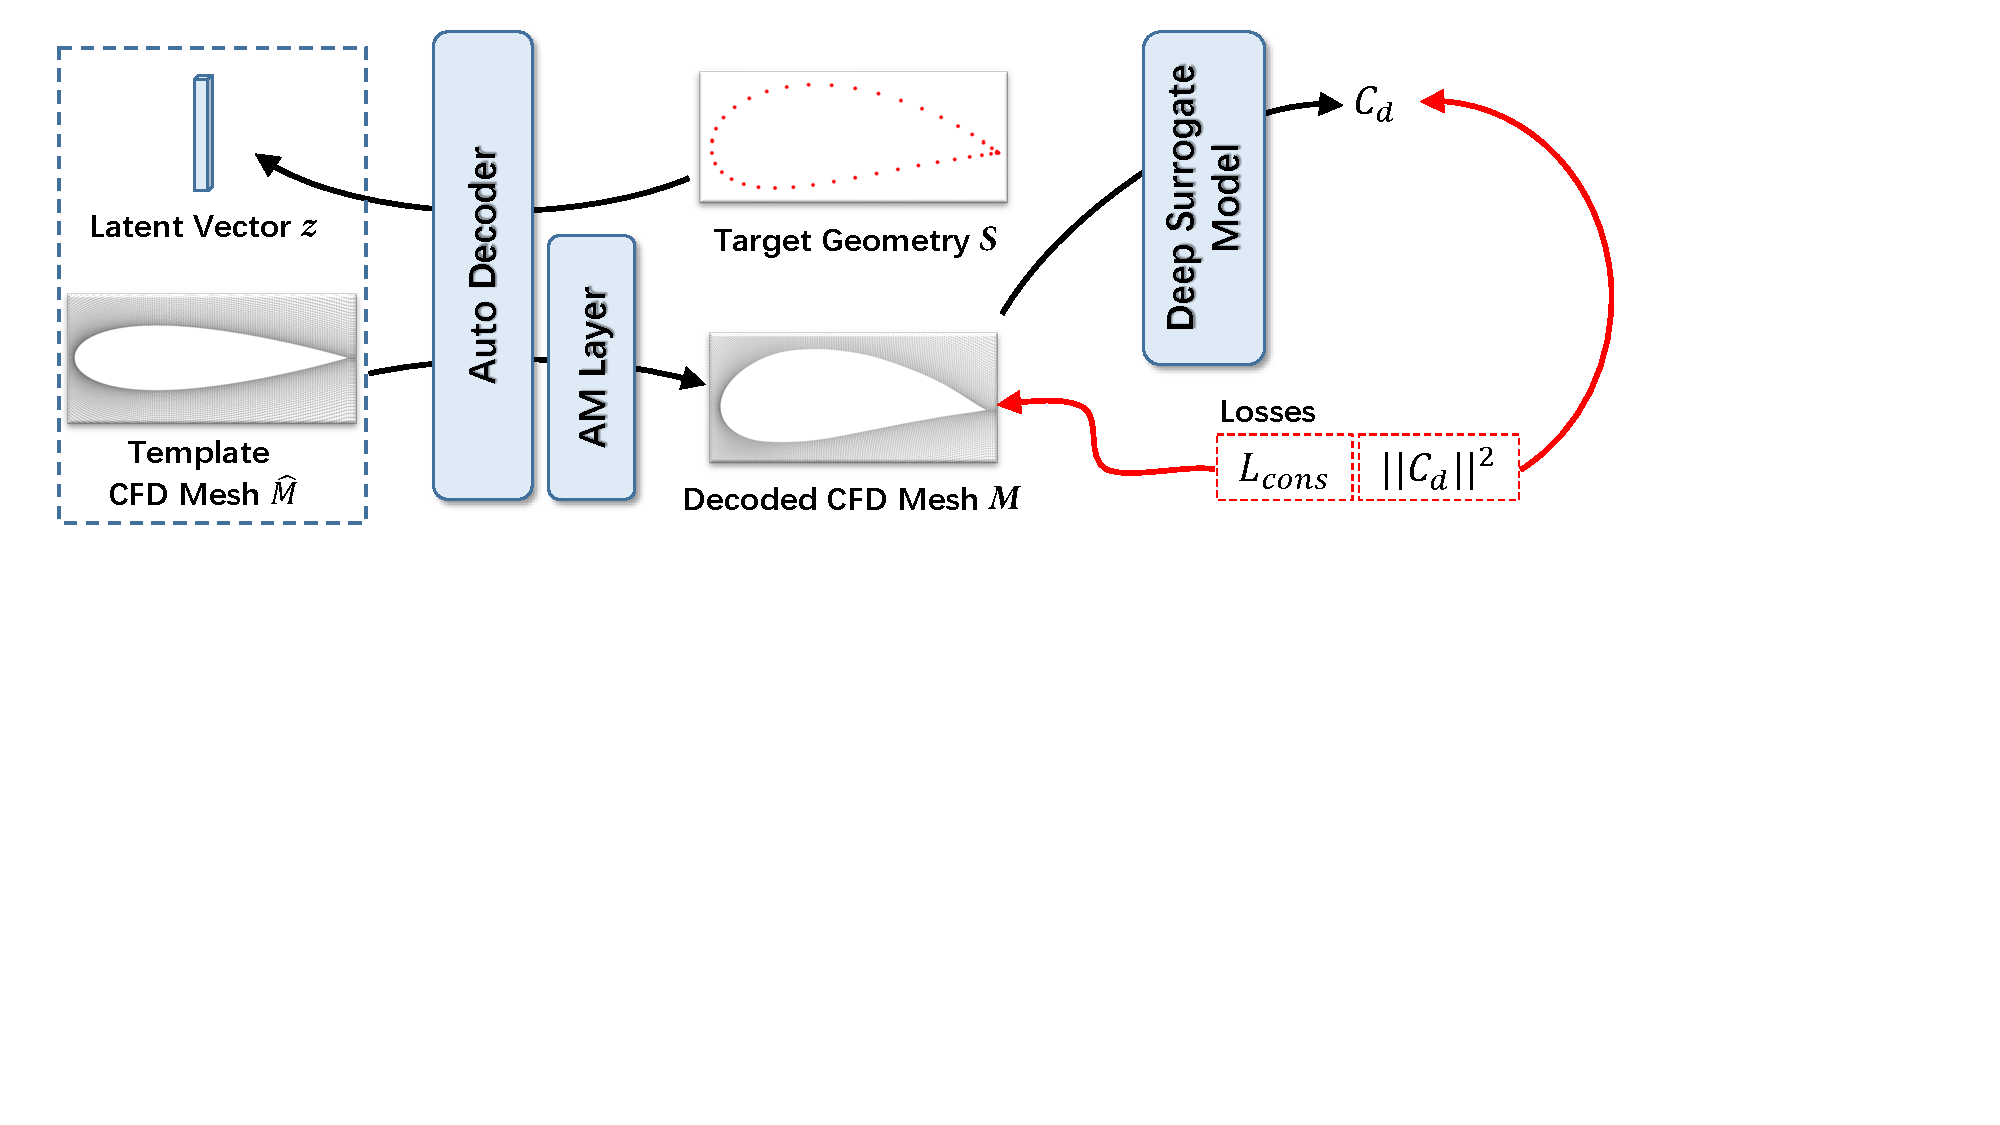
\includegraphics[width=0.95\linewidth]{chapter3/tex/figures/experiment/shape_optimization_pipeline.pdf}
	\end{center}
	\caption{
		\small The pipeline of shape optimization to minimize drag.
	}
	\label{ch3:fig:exp_shape_optim_pipeline}
\end{figure}

\begin{figure}[htb]
	\begin{center}
		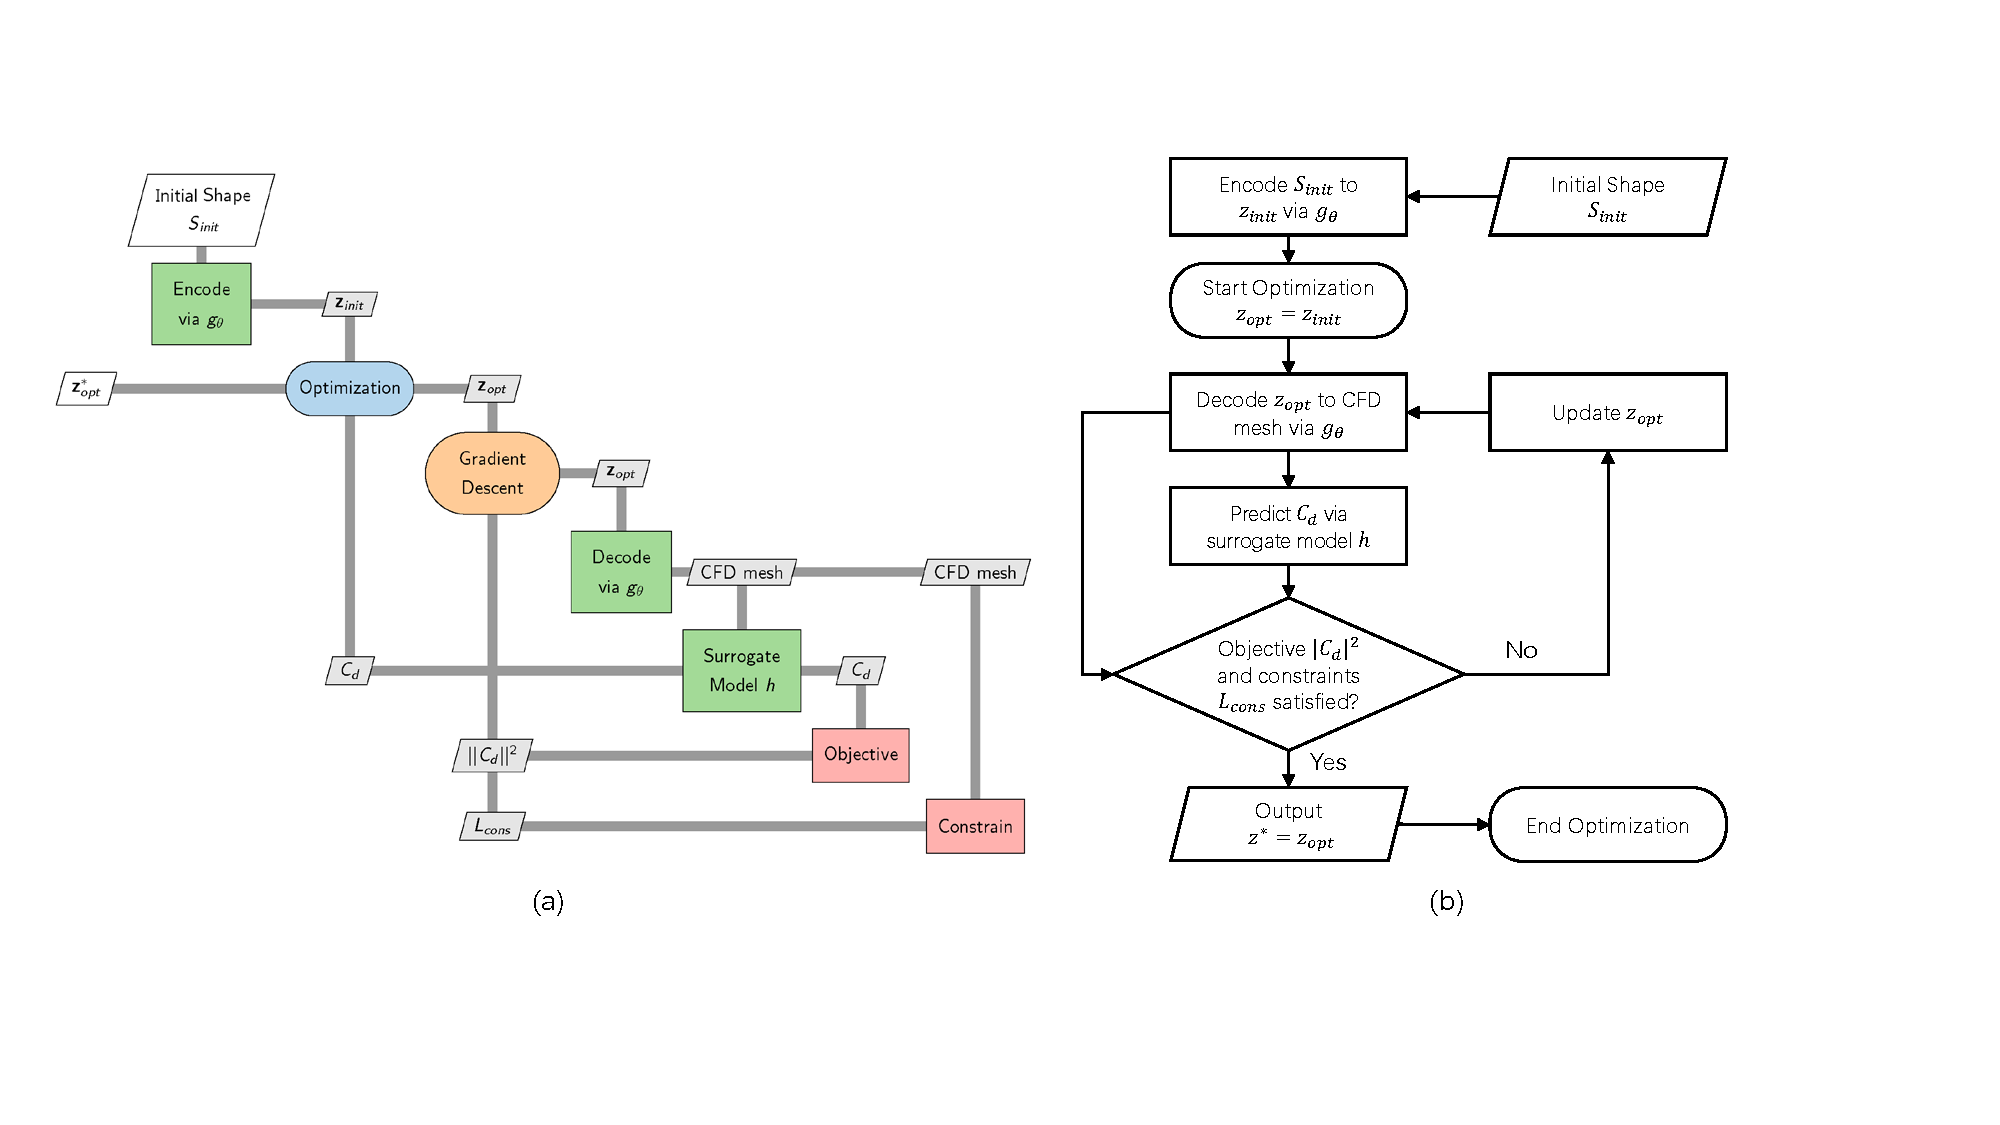
\includegraphics[width=1.02\linewidth]{chapter3/tex/figures/experiment/XDSM_flowchart.pdf}
	\end{center}
	\caption{
		\small The workflow of shape optimization shown in (a) the XDSM and (b) the flow chart.
	}
	\label{ch3:fig:exp_shape_optim_flow}
\end{figure}


\noindent \textbf{Pipeline Design.}
To implement a shape optimization pipeline, a surrogate model is required to evaluation the CFD properties of an airfoil.
There are multiple options for the surrogate model.
For example, the user can utilize an adjoint CFD solver (e.g. ADflow\cite{aa.Mader2020}, SU2\cite{aa.Economon2016}, etc.) to generate gradients by directly simulating on the reconstructed CFD mesh.
The user can also choose a deep learning model as the surrogate model.
Here we follow \cite{aa.Baque2018} and use a graph convolutional neural network (GCNN) to predict the air pressure on the airfoil's surface.
The pipeline is depicted by Fig.\ref{ch3:fig:exp_shape_optim_pipeline}.
More details of the surrogate model can be found in \textit{Appendix\ref{ch3:sec:appendix_surrogate}}.
We follow the surrogate-based optimization (SBO) scheme and the GCNN surrogate model needs to be re-trained by adding newly optimized results into the training set.
Our model reconstructs CFD meshes of new samples for CFD simulations.

\noindent \textbf{Optimization.}
The workflow of optimization is shown in Fig.\ref{ch3:fig:exp_shape_optim_flow}.
Given an initial airfoil, we first encode $S_{init}$ into a latent vector $\bz_{init}$ by Eq.\ref{ch3:eq:autodec}.
The latent code to be optimized $\bz_{opt}$ is initialized by $\bv_{init}$.
Then we fix the auto-decoder $g_\Theta$ as well as the trained GCNN surrogate model $h$, and optimize $\bz_{opt}$ by minimizing the predicted drag coefficient $C_d$ as
\begin{equation}
    \bz_{opt}^* = \mathop{argmin}\limits_{\bz_{init}} ||C_d||^2\,,\,\, \text{where} \,\,\,C_d = h(\hat{V} + g_\Theta(\bz_{init}), \hat{E}).
    \label{ch3:eq:optim_without_constrain}
\end{equation}

The optimized geometry can be extracted from the decoded mesh as
\begin{equation}
    V^S_{opt} \in V_{opt} = \hat{V} + g_\theta(\bz_{opt}).
\end{equation}

The Adam optimizer is used.
The maximum number of iteration is $300$ to ensure the convergence.

\begin{figure}[htb]
	\begin{center}
		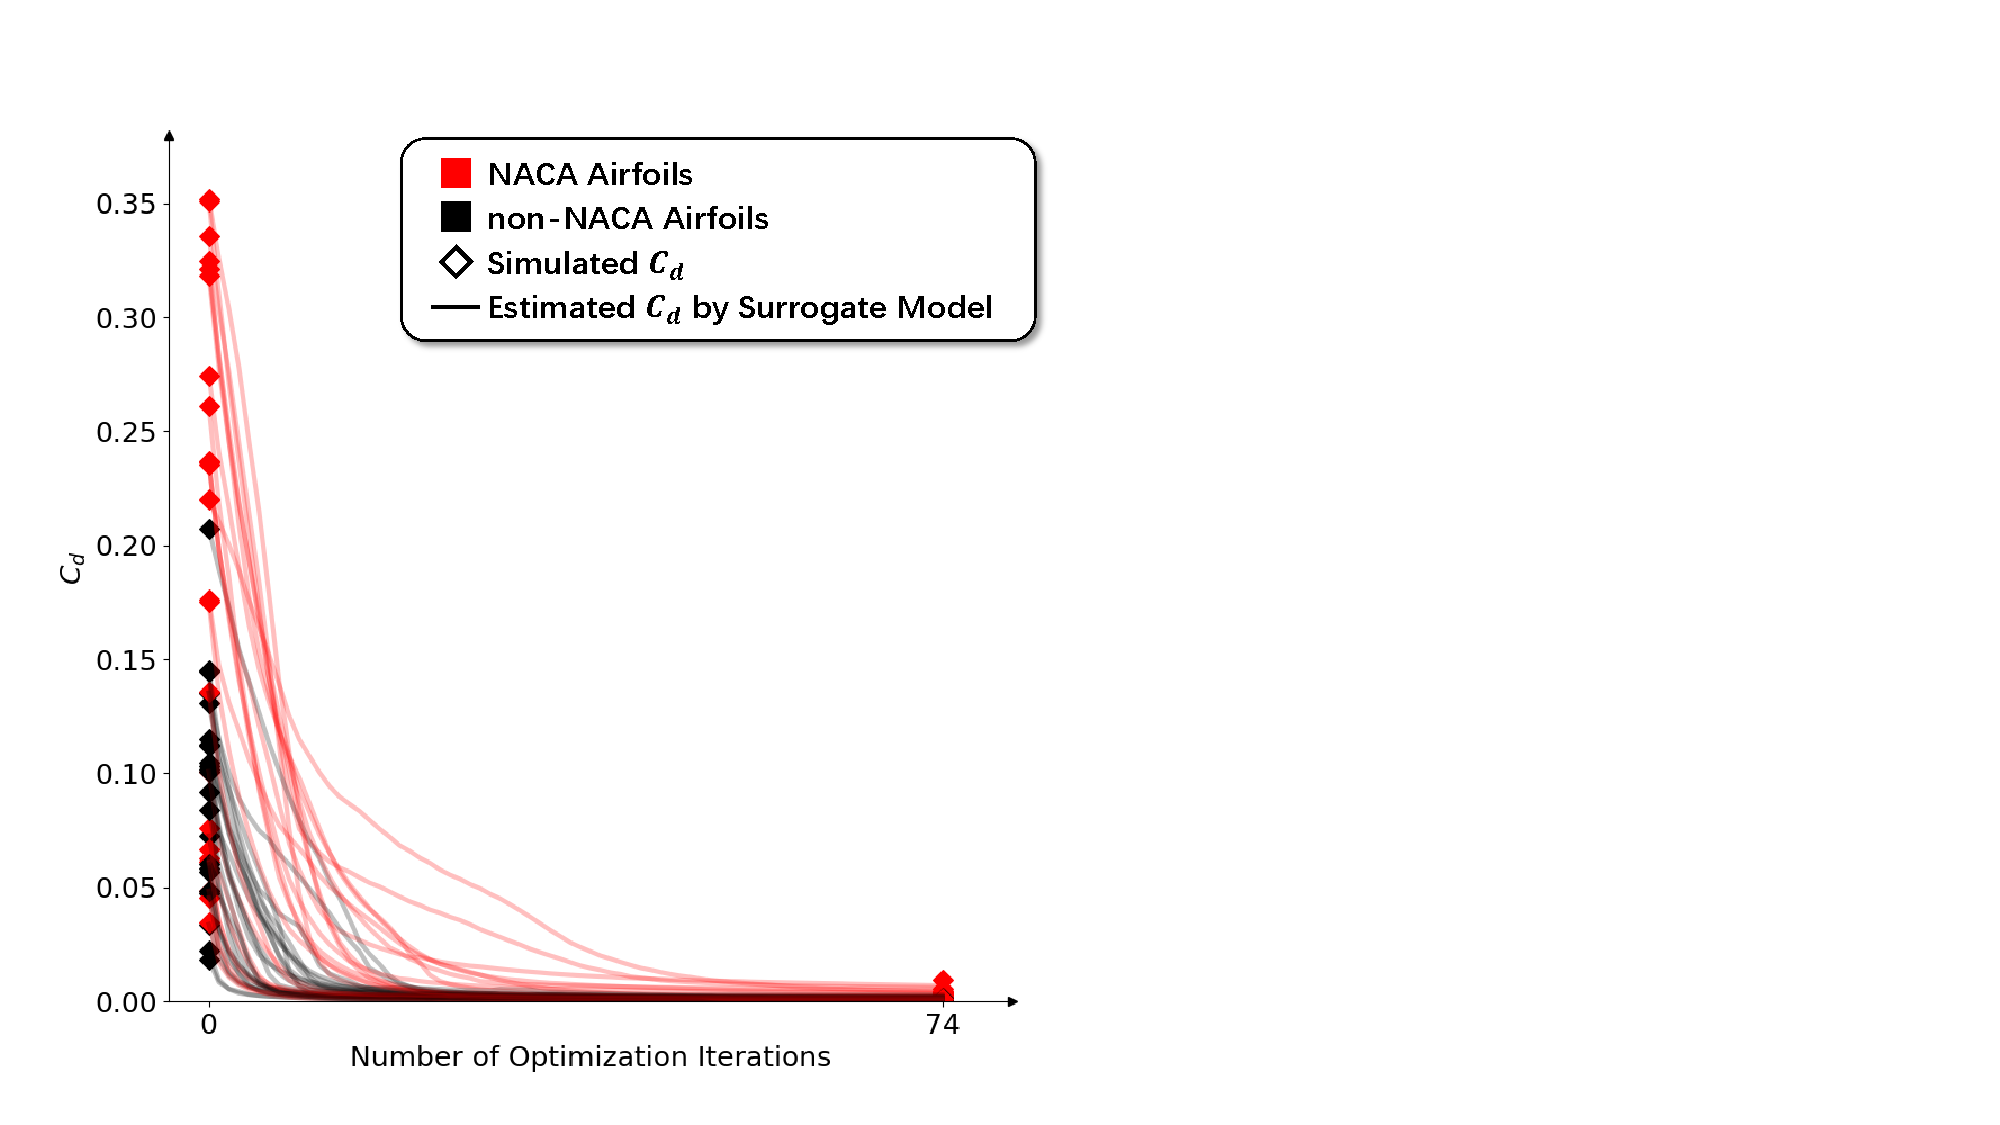
\includegraphics[width=0.6\linewidth]{chapter3/tex/figures/experiment/shape_optimization_batch.pdf}
	\end{center}
        \vspace{-2mm}
	\caption{
		\small The initial and optimized $C_d$ of 25 NACA and 25 non-NACA test airfoils.
	}
	\label{ch3:fig:exp_shape_optim_batch}
\end{figure}

\begin{figure}[htb]
	\begin{center}
		
        \vspace{-2mm}
        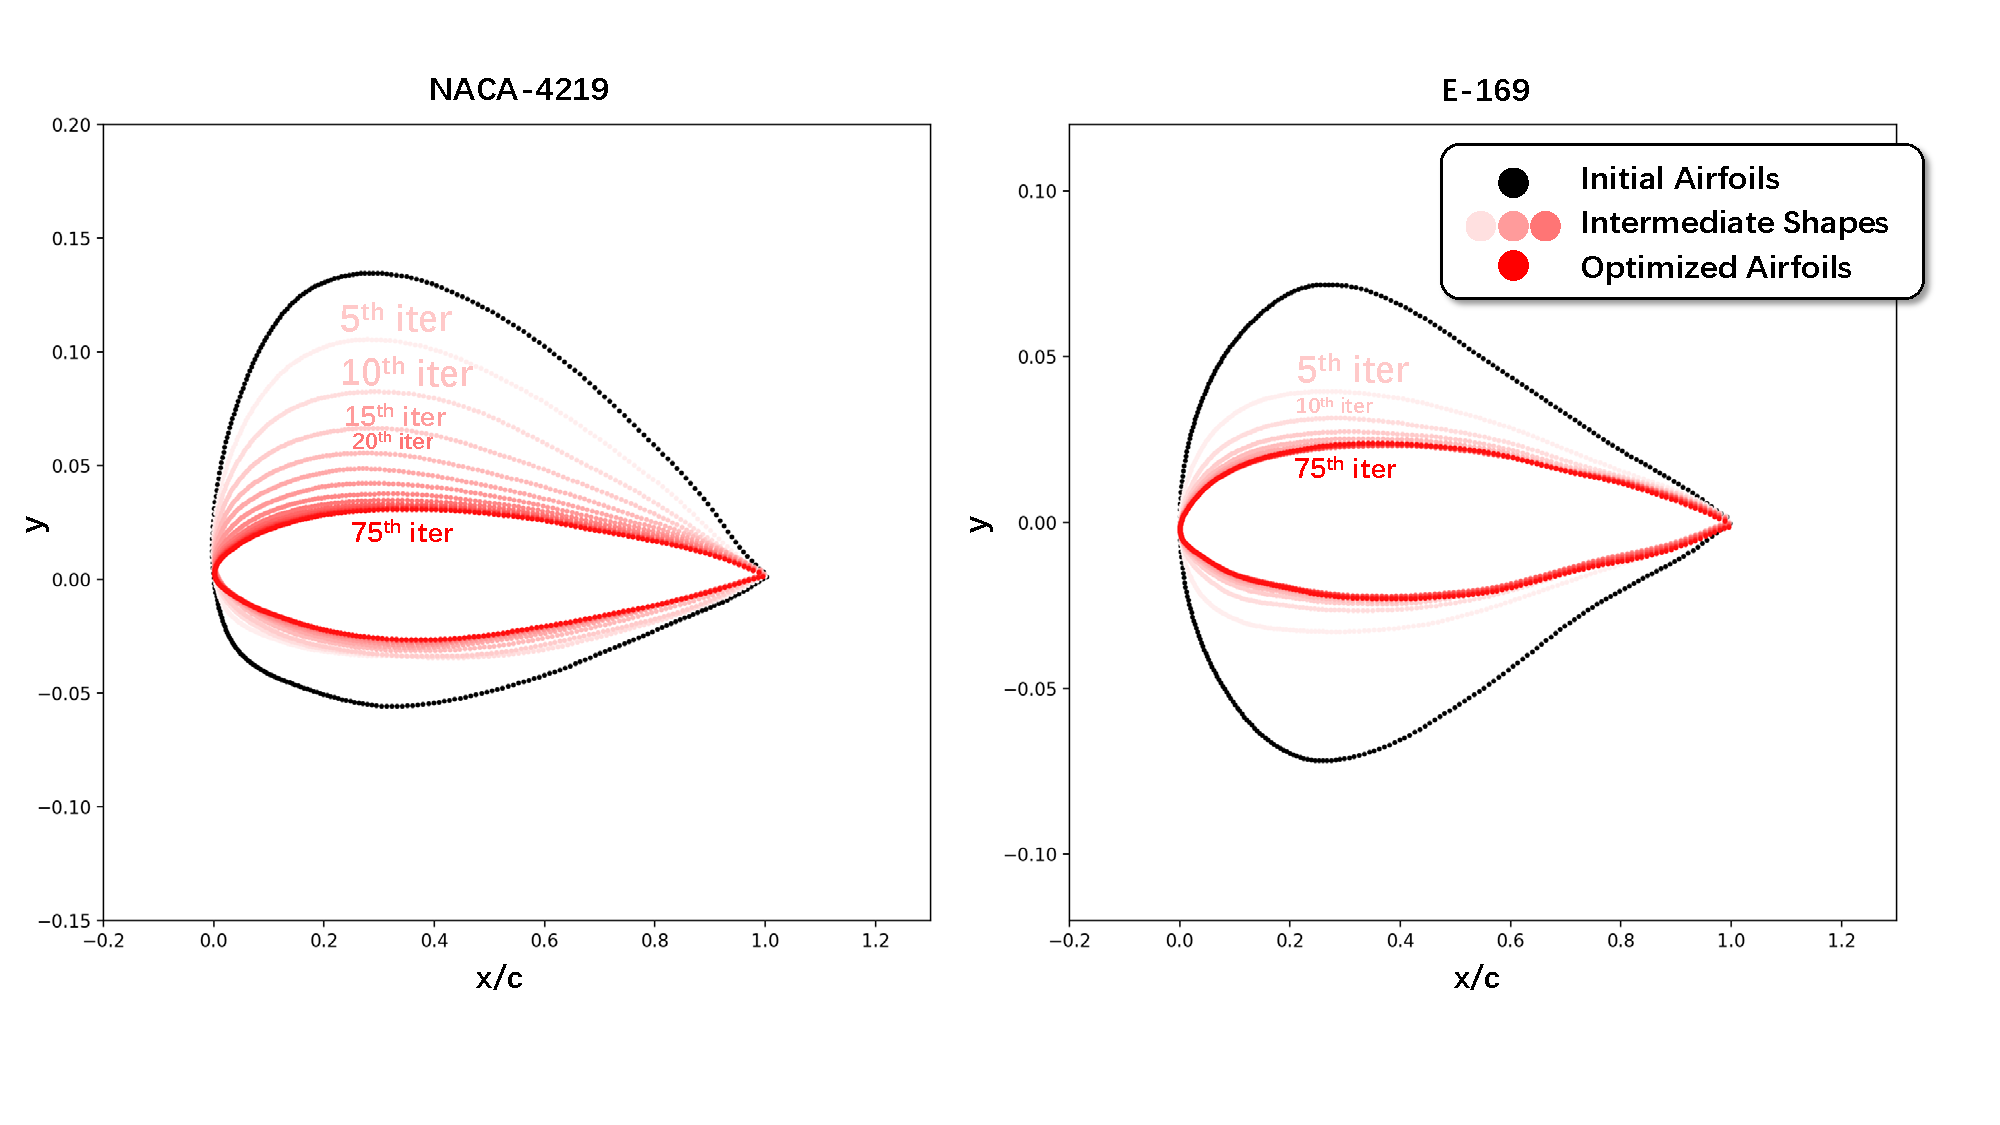
\includegraphics[width=0.9\linewidth]{chapter3/tex/figures/experiment/shape_optimization_batch_evolve.pdf}
	\end{center}

        \vspace{-2mm}
	\caption{ \small
		The evolution of airfoils during unconstrained shape optimization. Shapes are plotted at every five iterations.
	}
	\label{ch3:fig:optim_batch_evolve}
\end{figure}

\noindent \textbf{Results.}
We randomly collect $25$ NACA and $25$ non-NACA airfoils as initial shapes.
Optimizations are run on all airfoils and we simulate with OpenFOAM on the deformed shapes before the first iteration and after the last iteration to get their initial and optimized $C_d$ values.
Fig.\ref{ch3:fig:exp_shape_optim_batch} shows that the $C_d$s have been significantly reduced in all cases.
The model has consistent performances on NACA and non-NACA airfoils even when the mesh representation model is trained with NACA airfoils only.
On both airfoil series, the optimization on a single case takes 3.7s -- 4.2s.

Fig.\ref{ch3:fig:optim_batch_evolve} depicts the evolution of the airfoils during unconstrained shape optimization in two different cases, one initialized with NACA-4219 and the other with E-169. The shapes evolve from the initial black airfoils and progress as the shapes change from pink to red in color.

\subsubsection{Case Studies on Shape Optimization with Geometric Constraints}
In practice, the shape optimization problem is often coupled with certain geometric constraints.
These constraints are easy to integrate in our pipeline.
As shown in Fig.\ref{ch3:fig:exp_shape_optim_pipeline}, the constraints can be written as differentiable formula and regarded as an extra loss function $\cL_{cons}$.
$\cL_{cons}$ is applied directly on the deformed geometry. Eq.\ref{ch3:eq:optim_without_constrain} can be rewritten as
\begin{equation}
    \bz_{opt}^* = \mathop{argmin}\limits_{\bz_{opt}} ( ||C_d||^2 + w_{cons} \cL_{cons} )\,.
\end{equation}

In this section, we demonstrate optimization results with three different constraints, namely the bounding constraint, the maximum thickness constraint and the area constraint.
The bounding constraint limits the airfoil's thickness to be no less than the initial one, which is defined as
\begin{equation}
    {\cL_{cons}} = \frac{1}{{|{V^S}|}}\sum\limits_{i = 1}^{|{V^S}|} \left|\left|{\max (|y_i^{opt}| - |y_i^{init}|,0)}\right|\right|^2
    \,\,,\,\, \text{where}\,\,
    \left\{ 
        \begin{matrix}
      v_i^{opt} = (x_i^{opt},y_i^{opt}) \in V_{opt}^S \hfill \cr 
      v_i^{init} = (x_i^{init},y_i^{init}) \in V_{init}^S \hfill \cr 
        \end{matrix}
  \right.
  \,\,.
\end{equation}

\begin{figure}[!thb]
	\begin{center}
		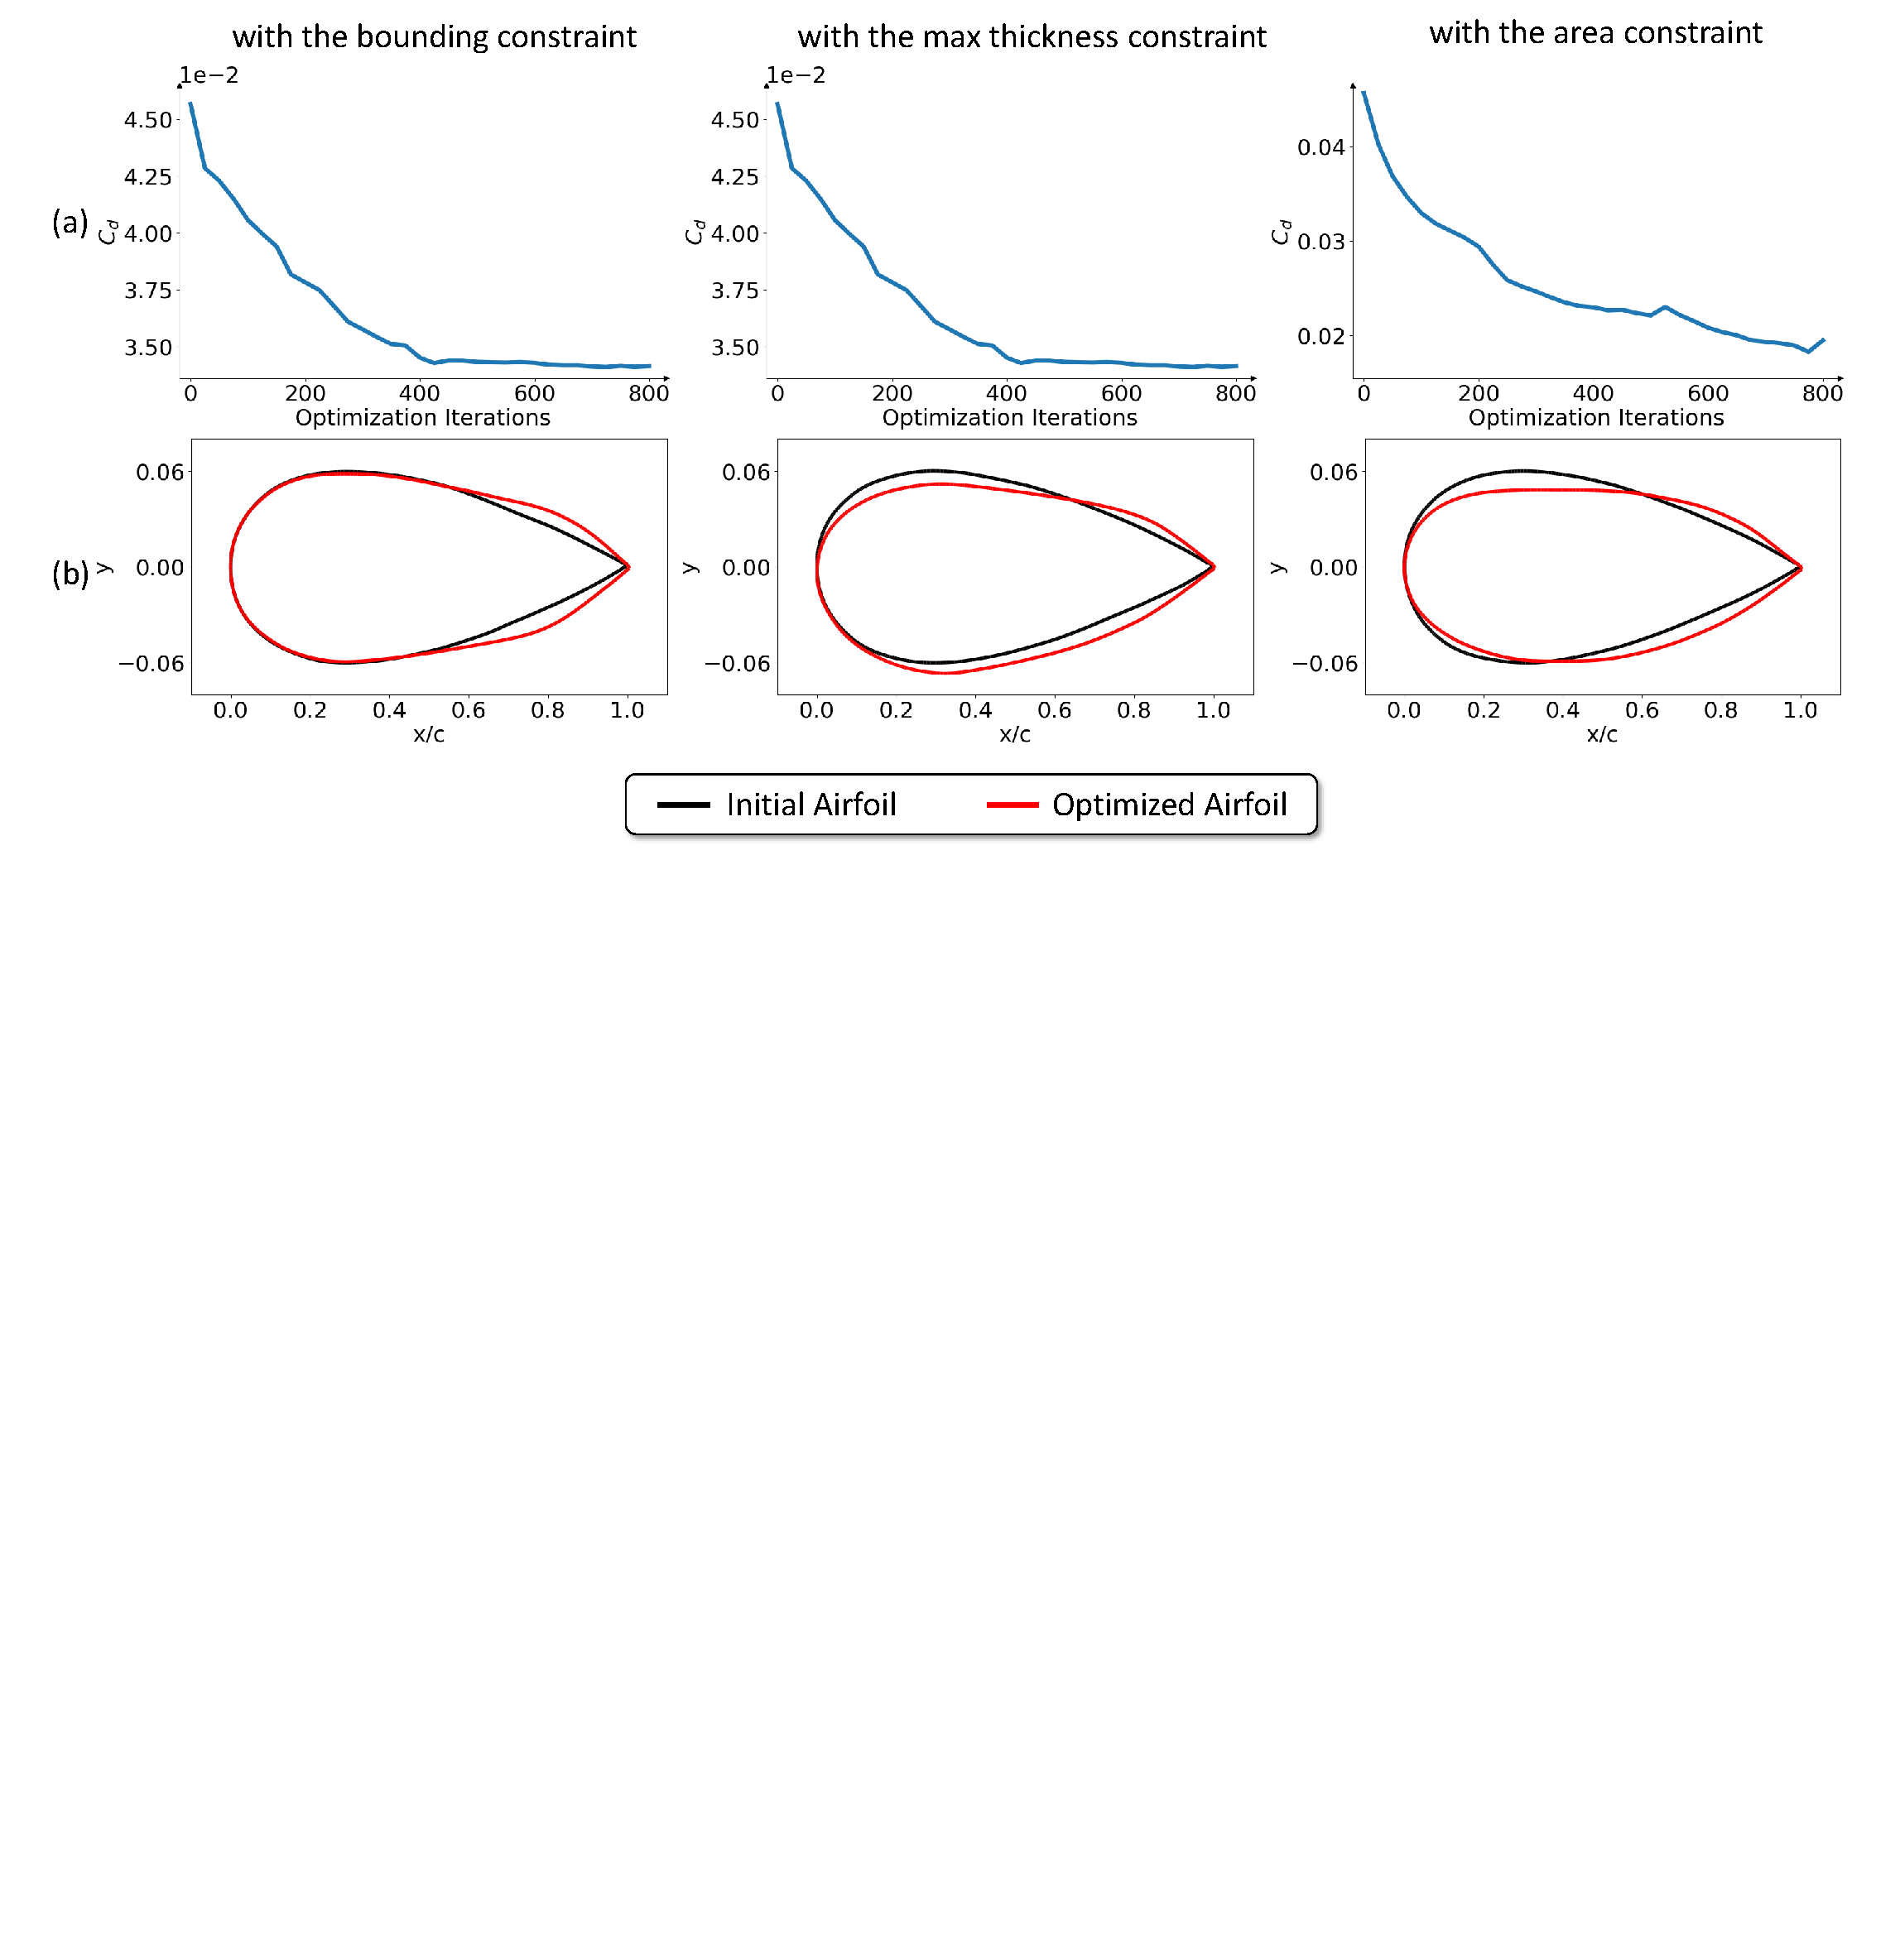
\includegraphics[width=1\linewidth]{chapter3/tex/figures/experiment/shape_optimization_case.pdf}
	\end{center}
	\caption{
		\small Optimized NACA-0012 with different geometric constraints. (a) Changes of $C_d$. (b) Changes of the airfoils.
	}
	\label{ch3:fig:exp_shape_optim_case}
\end{figure}

The maximum thickness constraint is a relaxed bounding constraint, which only limits the airfoil's maximal thickness.
To implement it, we use cubic splines, $spline^+(\cdot)$ and $spline^-(\cdot)$, to interpolate the surface positions on the upper airfoil and lower airfoil given a horizontal coordinate $x$, and then calculate the thickness by subtracting the vertical coordinates.
Considering that airfoils' chord lengths are $1$ and the leading edges are placed at the origin, then the constraint can be written as
\begin{equation}
    {\cL_{cons}} = \mathop {\max }\limits_{x \in (0,1)} \left( {\left|\left|\max ((spline_{init}^ + (x) - spline_{init}^ - (x)) - (spline_{opt}^ + (x) - spline_{opt}^ - (x)),0)\right|\right|^2} \right)\,\,.
\end{equation}

The area constraint is to limit the optimized airfoil's area to be no less than the initial one.
We use the Shoelace formula to compute the airfoil's area $A$.
By sorting $V^S$ in clockwise order, the constraint is
\begin{equation}
    {\cL_{cons}} = \left|\left|\max (A_{init}(V_{init}^S) - A_{opt}(V_{opt}^S),0)\right|\right|^2\,,\,\,\text{where}\,\,A({V^S}) = \frac{1}{2}\sum\limits_{i = 1}^{|{V^S}|} {{y_i}({x_i} - {x_{i + 1}})} \,\,.
    \label{ch3:eq:constraint_area}
\end{equation}

We use NACA-0012 as the initial airfoil and perform three optimizations with the geometric constraints in mention.
The optimized results are demonstrated in Fig.\ref{ch3:fig:exp_shape_optim_case}.
In all cases the drag coefficients are reduced by a noticeable proportion and the geometric changes are explainable under the inviscid flow condition.
The optimized airfoils move the shock waves towards its trailing edge under all constraints.
They change the directions of surface normal near the trailing edge so as to counteract the drag forces generated at the leading edge.
Meanwhile, the area constraint relaxes the limitation on airfoil's thickness so that the airfoil's leading edge is narrowed to reduce drag.

\begin{figure}[!htbp]
    \begin{center}
    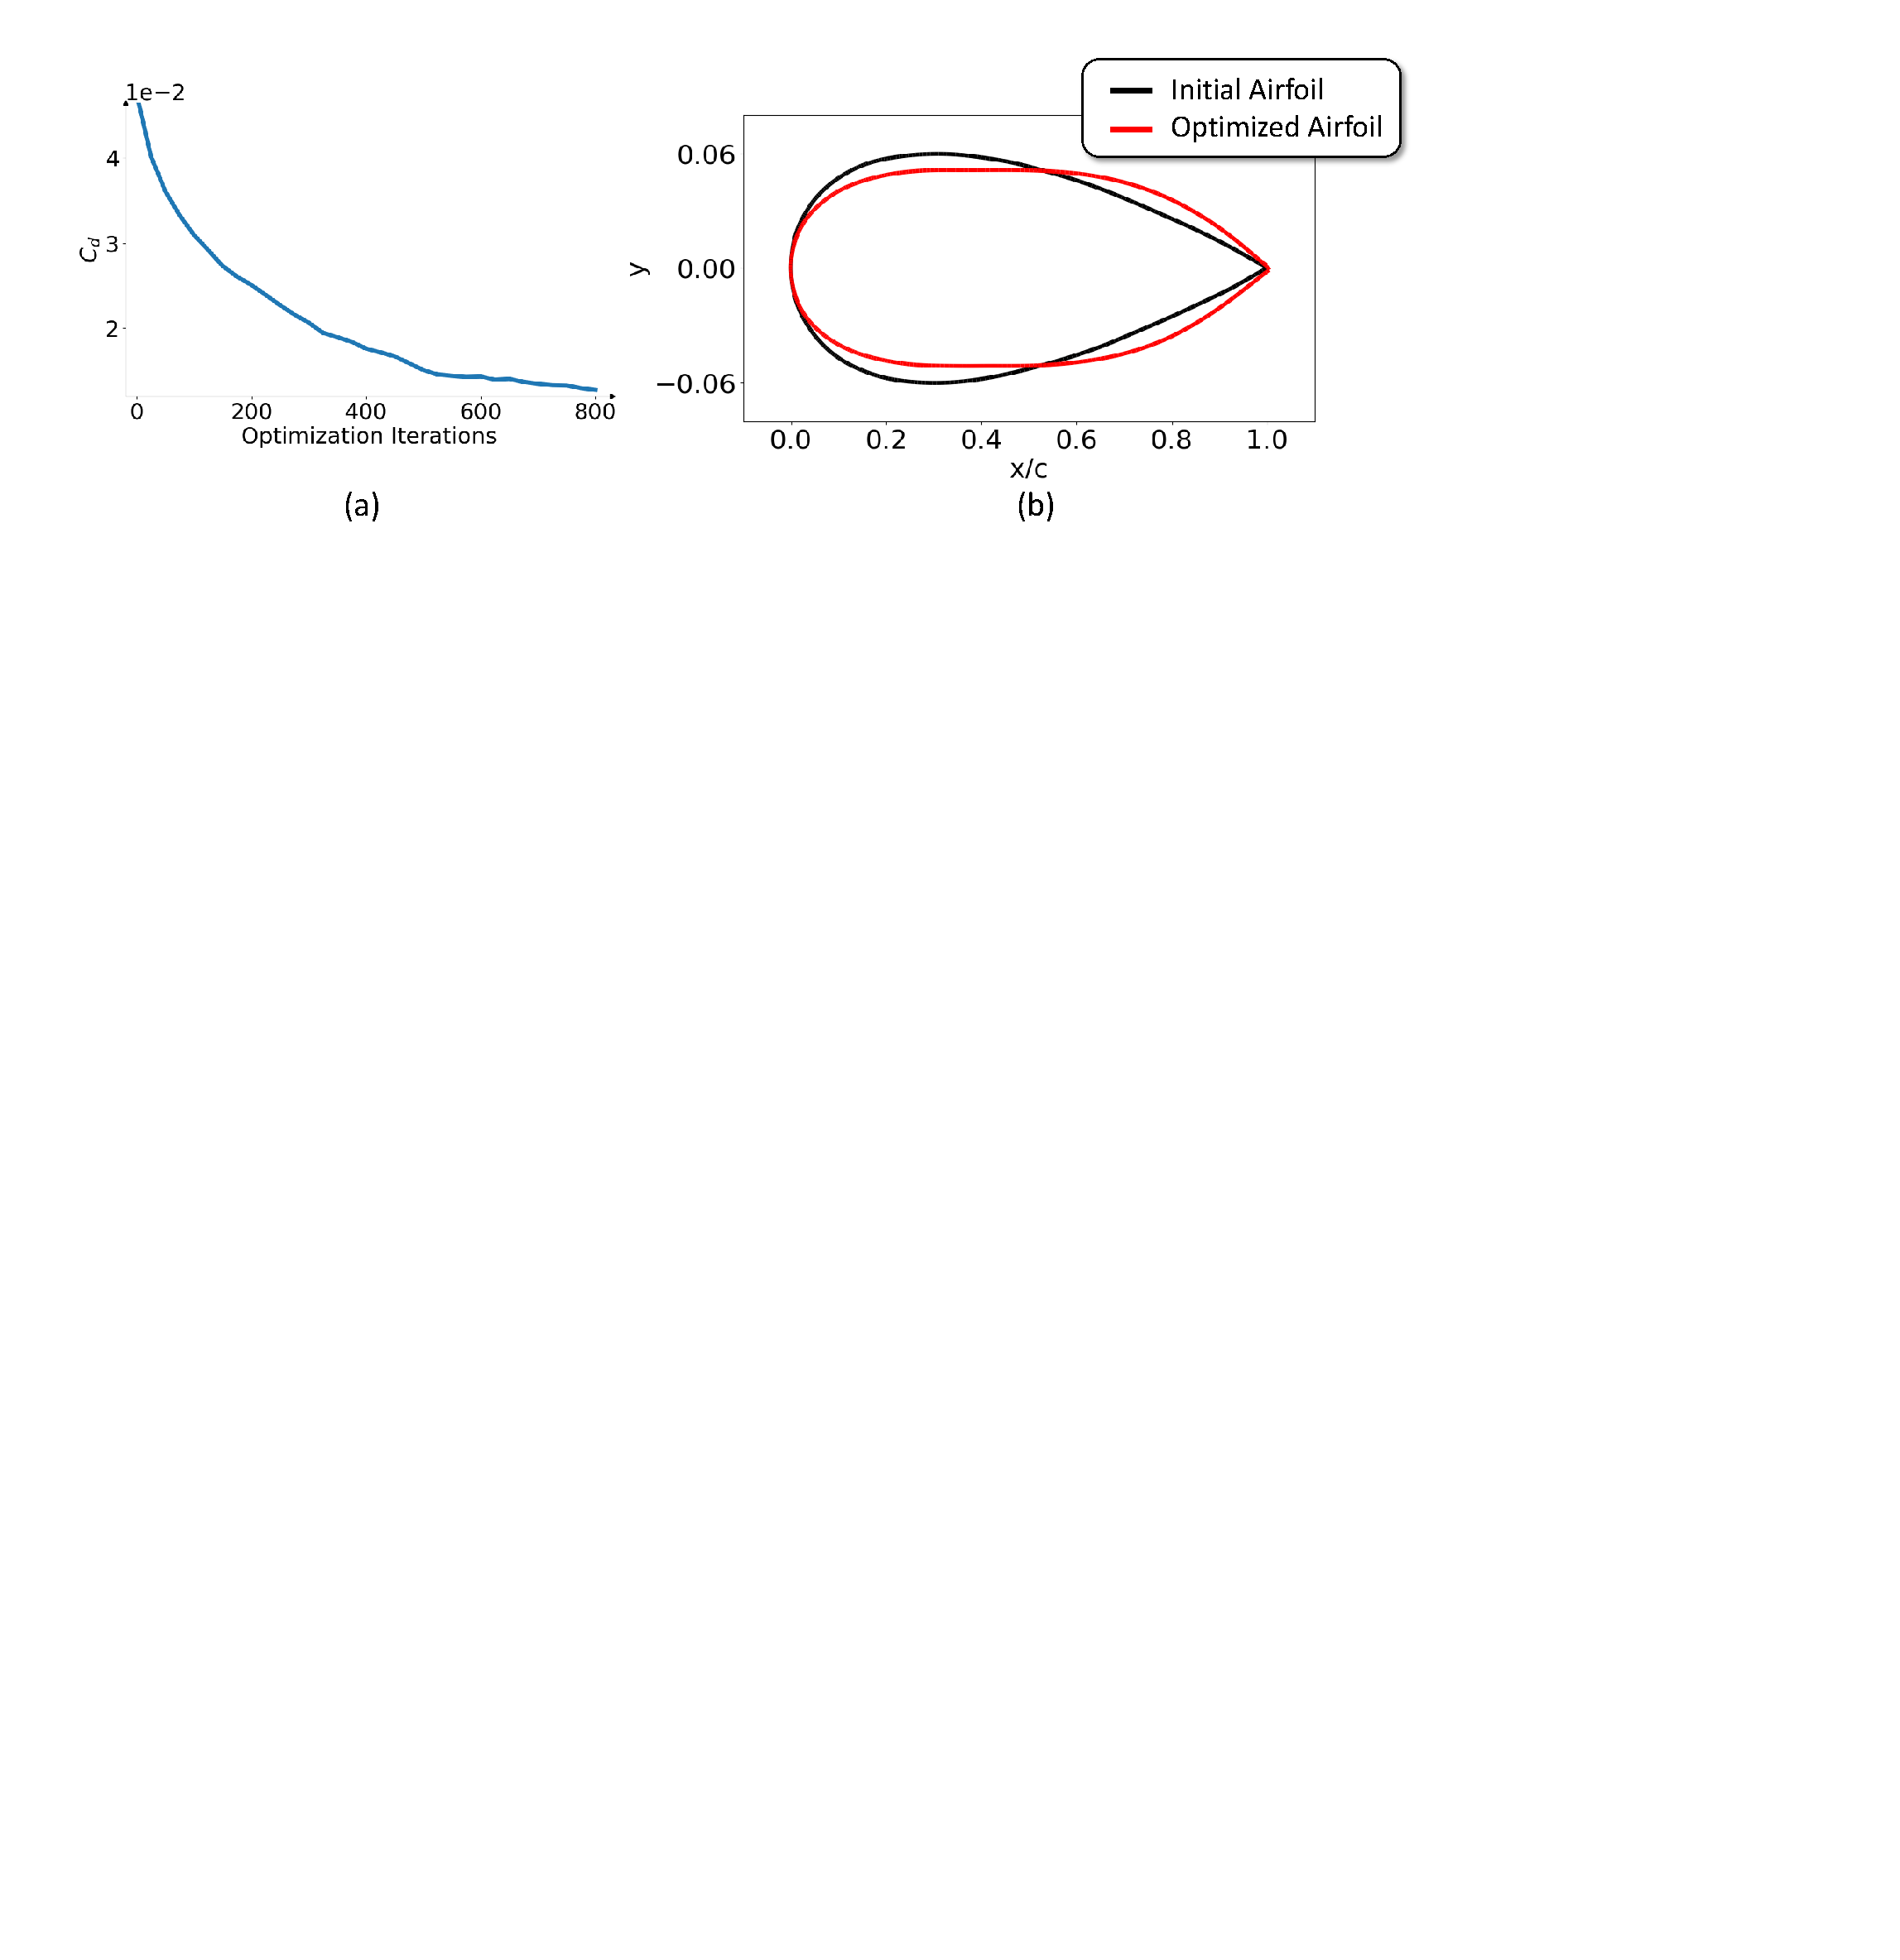
\includegraphics[width=0.9\linewidth]{chapter3/tex/figures/experiment/shape_optimization_case_2_constraints.pdf}
    \end{center}
    \caption{ \small
		Optimized NACA-0012 with the area and symmetry constraints. (a) Changes of $C_d$. (b) Changes of the airfoil.
    }   
    \label{ch3:fig:exp_optim_2_constraints}
\end{figure}

The full differentiation of our mesh model, along with our  end-to-end trainable pipeline, makes it possible to easily handle multiple constraints. For example, we combine the area constraint defined by Eq.\ref{ch3:eq:constraint_area} and a symmetry constraint that ensures the consistency between airfoil's upper and lower curves. Then $L_{cons}$ is the simple addition of both constraints, which writes

\begin{align}
    \begin{split}
        {\cL_{cons}} = \left|\left|\max (A_{init}(V_{init}^S) - A_{opt}(V_{opt}^S),0)\right|\right|^2 &+{\left|\left|\,\left|spline_{opt}^ + (x)\right| - \left|spline_{opt}^ - (x)\right|\,\right|\right|^2}\,\,,\\
        &\text{where}\,\,A({V^S}) = \frac{1}{2}\sum\limits_{i = 1}^{|{V^S}|} {{y_i}({x_i} - {x_{i + 1}})} \,\,\text{and}\,\, x\in(0,1)\,.
    \end{split}
\end{align}

The result of Fig.\ref{ch3:fig:exp_optim_2_constraints} shows that the optimized shape satisfies both constraints without compromising the performance on reduced drag.

In summary, the results show that our model is effective for the fast prototyping of object shape designs and is able to work in a fully automatic fashion.